% don't remove the following lines, and edit the definition of \main if needed
\documentclass[../report.tex]{subfiles}
%\usepackage[utf8]{inputenc}
\providecommand{\main}{..}
\IfEq{\jobname}{\currfilebase}{\AtEndDocument{\biblio}}{}
% until here



%defined commends for flow section
\providecommand*{\psin}{\ensuremath{\Psi_{n}}}
\providecommand*{\ppb}{\ensuremath{p}+Pb}
\providecommand*{\pbpb}{Pb+Pb}
\providecommand*{\pt}{\ensuremath{p_{\mathrm{T}}}}
\providecommand*{\vn}{\ensuremath{v_{\mathrm{n}}}}



\begin{document}

\section{Flow and Correlations}

\noindent \textbf{Coordinators}: Soumya Mohapatra (Columbia University)


\noindent \textbf{Contributors}: Alexandru Florin Dobrin (CERN), Stefan Floerchinger (University of Heidelberg), Wei Li (Rice University), Vitaly Okorokov (National Research Nuclear University MEPhI), Bjoern Schenke (Brookhaven National Lab)

Charm and beauty quarks are produced in hard scattering processes occurring in the early stage of heavy-ion collisions. They subsequently traverse the QGP medium and interact with its constituents through inelastic (gluon radiation) and elastic (or collisional) processes.
These interactions may lead to the thermalisation of low-momentum heavy quarks, which would thus take part in the expansion and hadronisation of the medium.
For these reasons, heavy-flavour hadrons provide information on all stages of the system evolution and they uniquely probe the quark-mass dependence of the QGP inner workings (see Refs.~\cite{Andronic:2015wma,Prino:2016cni,Rapp:2018qla} for recent reviews).

Many experimental observations from RHIC and LHC showed evidence that charm and beauty quarks interact strongly with the QGP and that beauty quarks lose less energy at low transverse momentum compared to charm quarks~\cite{Adam:2015nna,Khachatryan:2016ypw}. 
While data are becoming more and more precise to start imposing constraints on theoretical calculations, there are still several unresolved questions: What are the microscopic mechanisms that drive heavy-flavour interaction and diffusion in the QGP, and what are their implications for the QCD matter structure? What is the relative relevance of collisional and radiative processes? Are their relations between the interactions giving rise to the strongly coupled QGP and hadronisation?
%What is the relative importance of radiative and collisional energy loss, and their parton mass dependence? 

The Run 3 and 4 of the LHC will open a new precision era for heavy-flavour measurements in heavy-ion collisions that will address the above questions.
With the upgrades of the machine and of the tracking detectors, the higher accumulated statistics and higher precision will make it possible to quantify the properties of the QGP with heavy-flavour probes. This high-precision era will also make new and more differential observables accessible for the first time.
The key measurements that are expected to have a strong impact on the characterisation of the QGP with heavy-flavour observables are discussed in this chapter and summarized below.
\begin{itemize}
\item Nuclear modification factor and flow harmonics: these measurements for particles with charm and beauty in the large kinematic range covered by combining the different LHC experiments will put the strongest constraints on the transport coefficients of the QGP, clarifying the microscopic mechanisms governing the interactions of heavy quarks with the medium, and quantifying their degree of thermalisation.
\item Strange D and B mesons, charm and beauty baryons: currently limited by statistics, these measurements will help to quantify not only the degree of thermalisation of heavy quarks, but also the contribution of recombination with lighter quarks to the hadronisation process. They are also sensitive to the mass scaling of the hyrodynamical flow in the heavy-flavour sector.
\item Heavy-flavour correlations and jet observables: they will provide new insights on the parton mass effects in parton showers, on the redistribution of the radiated energy, and on the role of collisional and radiative energy loss.

\end{itemize}


 %Bjoren,Stefan +(Soumya)
\FloatBarrier
\subsubsection{Identified particle \vn}\label{sec:identified_particle_vn}


\begin{figure}[!htb]
\begin{center}
\includegraphics[width=0.495\textwidth]{\main/flow/figs/alice_projection_pid_v2}
\includegraphics[width=0.495\textwidth]{\main/flow/figs/alice_projection_pid_v3}
\caption{
ALICE projections for $v_2$ (left) and $v_3$ (right) of $\pi^\pm$, 
  $\mathrm{p}$+$\overline{\mathrm{p}}$, $\Xi$+$\overline{\Xi}$, 
  $\Omega$+$\overline{\Omega}$, and the $\phi$-meson 
  in the 10--20\% centrality interval
  for an integrated luminosity of 10~nb$^{-1}$. 
Error bars (shaded boxes) represent the projected statistical 
  (systematic) uncertainties.}
\label{fig:alice_vn}
\end{center}
\end{figure}

As stated earlier most traditional \vn\ measurements (event-plane or 
  two-particle correlation) for inclusive hadrons at the LHC 
  are not statistics limited.
However for identified particles there is considerable scope for reduction 
  in statistical uncertainties in Run~3 and 4.
This is true both for heavy-flavor particles (discussed further in Chapter~\ref{sec:HI_HF})
  for heavy-flavor particles and their physics implications. 
  as well for identified light flavour hadrons.
Figure~\ref{fig:alice_vn} shows projections from the ALICE collaboration for 
  the $v_2$ and $v_3$ of several light-flavor species, that are expected for 
  an integrated luminosity of 10~nb$^{-1}$ expected in Run~3 and 4.
The projected statistical uncertainties are typically negligible over the 
  entire \pt\ range and in most cases the systematic uncertainties are 
  quite small as well.

As stated before, the increased precision of these measurements will help in 
  better understanding of the QGP equation of state. 
These measurements will also lead to an improved understanding 
  of the hadronization mechanism at the QGP$\rightarrow$hadron transition.
Additionally, detailed measurements of constituent quark scaling (or its violation)
  can provide constraints on the contribution of the subsequent hadronic 
  rescattering, to the final azimuthal anisotropy of the final particles.
This is because the azimuthal anisotropy developed in the QGP phase 
  is expected to scale with the 
  number of constituent quarks, while the anisotropy developed in the hadronic
  phase is different for different particle species, depending on the particle 
  mass and hadronic coss-section.


%\begin{figure}[!htb]
%\begin{center}
%\includegraphics[width=1.0\textwidth]{\main/flow/figs/atlas_hfmuonv2}
%\caption{
%ATLAS projections of $v_2$ as a function of \pt, for muons from the decay of 
%  heavy-flavor hadrons. 
%Each panel corresponds to a different centrality interval. 
%The present measurements are also shown for comparison. 
%The error bars (shaded boxes) correspond to statistical uncertainties only. 
%The projections are also compared to calculations from the DABMod model.}
%\label{fig:atlas_hf_v2}
%\end{center}
%\end{figure}
%
%Figure~\ref{fig:atlas_hf_v2} shows projections from the ATLAS collaboration
%  for the $v_2$ of muons produced from the decay of heavy-flavor hadrons
%  in Run~3 and 4, showing a considerable improvement in the statitical 
%  precision of the measurement.
%The central values of the projections are obtained by fitting the 
%  present measurements with an exponential function, which qualitatively 
%  describes the present data. 
%The statistical uncertainties in the projections are made by scaling down 
%  the present uncertainties to correspond to the expected luminosity in 
%  Run~3 and 4 (10~nb$^{-1}$).
%Calculations from the DABMod model~\cite{Prado:2016szr} are also shown,
%  which demonstrate the inability of the present measurements
%  in establishing or ruling out models due to limited statistical precision.
%The flow measurements for heavy quarks is important as they are produced at
%  earlier times in the heavy-ion collision and thus are susceptible
%  to the full time evolution of the QGP.
%The heavy-flavor anisotropy measurements can determine if heavy-quarks couple 
%  strongly or weakly to the QGP, and additionally can constrain the heavy-quark 
%  transport and diffusion coefficients.
%Chapter~\ref{sec:HI_HF} has further discussions of Run~3 and 4 flow projections
%  for heavy-flavor particles and their physics implications. 
%
%
%Bjoern, Stefan, Soumya
\FloatBarrier


\section{Initial conditions} \label{sec:initialstate}
As already alluded to in Section \ref{sec:macro}, the intial state of heavy ion collisions is the major source of uncertainty when it comes to extracting transport properties of the produced medium. This has to do with the fact that calculations of the exact geometry and its fluctuations involve nonperturbative physics. The available descriptions for the initial state thus range from very simplistic models that assign deposited energy densities based on the wounded nucleons or binary collisions determined in a Monte-Carlo Glauber prescription, to classical effective theories of QCD that are valid in the high energy limit. The latter are certainly closer to first principles calculations, and should provide a realistic description of the initial state assuming that the high energy limit is a good approximation.

The major ingredient that needs to be provided by an initial state model is the geometry of the interaction region in the plane transverse to the beam. It is entirely dominated by the positions of incoming nucleons whose fluctuations also play an important role. Observables are also sensitive to the detailed way the energy is deposited given a distribution of wounded nucleons, and the constraints on this from data are surprisingly robust \cite{Moreland:2018gsh}. Using the Trento model it was found that the product of thickness functions of the two nuclei at every given transverse position gives the best description of the data (compared to a conventinal wounded nucleon model or other combinations of thickness functions). This type of energy deposition is very much what the EKRT \cite{Niemi:2015qia} and IP-Glasma \cite{Schenke:2012wb,Schenke:2012fw} models include, explaining their success in describing a wide range of observables \cite{Niemi:2015qia,Gale:2012rq}.

Fluctuations of wounded nucleon positions contribute the dominant effect to fluctuations of the initial geometry in heavy ion collisions. Smaller scale fluctuations (emerging e.g. from color charge fluctuations in the IP-Glasma model) have been shown to not significantly affect most observables measuring the momentum anoisotropy of produced particles \cite{Gardim:2017ruc}. The factorization breaking ratio shows some sensitivity and it should be pointed out that multiplicity fluctuations are also influenced by the existence of color charge fluctuations.

More recently, indications that the nucleon should possess a substructure of hotspots have emerged. The IP-Glasma model was unable to describe flow coefficients in p+Pb collisions assuming a round proton \cite{Schenke:2014zha}. Including subnucleonic fluctuations constrained by incoherent diffractive $J/\psi$ production data from HERA \cite{Mantysaari:2016ykx} (which also require a fluctuating proton geometry) improved the agreement with the p+Pb data significantly \cite{Mantysaari:2017cni}. Recent Bayesian analyses also found that nucleon substructure is necessary to simultaneously describe p+Pb and Pb+Pb bulk observables \cite{Moreland:2018gsh}.
It should be noted, however, that the size scales for nucleons and subnuclear hot spots extracted in that work are significantly larger than those obtained from comparison to HERA data in the IP-Glasma model.

Initial conditions for hydrodynamic simulations have to provide, in principle, all components of the energy momentum tensor as a function of spatial position (and initial conditions for other conserved charges, if considered). This includes, apart from the always included energy density distribution, the initial flow as well as initial viscous corrections. Initial flow is included in many recently developed models, that either assume free streaming \cite{Moreland:2018gsh}, including Yang-Mills evolution, which is close to free streaming \cite{Gale:2012rq} or an initial flow distribution motivated by strong coupling calculations \cite{Weller:2017tsr}. Initial viscous corrections are often set to zero. Only a few works \cite{Mantysaari:2017cni,Schenke:2018fci,Moreland:2018gsh} include the full viscous stress tensor provided by the initial state description.

Since the initial state models that provide the entire $T^{\mu\nu}$ all switch from essentially a freely streming system to strongly interacting hydrodynamics at a fixed time $\tau$, that transition is somewhat abrupt and not very physical. To improve over this situation an intermediate step using effective kinetic theory has been introduced \cite{Kurkela:2018wud,Kurkela:2018vqr}. This procedure allows for a somewhat smoother matching but has yet to be used in full fledged hydrodynamic simulations. The effect on observables in heavy ion collisions is likely small, while in small systems, such as p+A a larger effect can be expected.

As already discussed in Section \ref{sec:macro}, the choice of initial state has a significant effect on the extraction of transport coefficients. A more compact initial state and the presence of initial flow lead to a larger transverse flow, which requires a larger bulk viscosity to compensate for it and produce agreement with experimental data \cite{Schenke:2018fci}. Also, the models' eccentricities will affect the final momentum anisotropies, influencing the extracted shear viscosity to entropy density ratio. Two possible attempts to solve this problem have been pursued: Constrain an initial state description as well as possible using data from experiments other than heavy ion collisions (e.g. e+p scattering data, which will hopefully be extended to e+A in a future electron ion collider facility), or perform a combined Bayesian analysis of all parameters, including those of the initial state, to find the best fit for all transport coefficients along with the initial state description.

As mentioned above, at the moment the two approaches lead to some similar features of the initial state (product of thickness functions, presence of subnucleon structure), but also show discrepancies (size of the nucleon and sub-nucleon scales along with the size of the extracted bulk viscosity). Only when the two methods converge for all features of the initial state and medium properties, can one confidently declare that the initial state as well as the transport properties of the QGP are understood.
\FloatBarrier
%\subsection{Introduction}
%\begin{itemize}
%	\item General introduction
%	\item Why is it interesting to study the fluid dynamics of the QGP
%	\item What has been learnt so far at LHC 
%	\item What questions remain
%\end{itemize}

\FloatBarrier
%%\subsection{Response functions}

% text from Stefan
%In a fluid dynamic description of heavy ion collisions,  one can understand the azimuthal harmonic flow coefficients $v_n$ as a response to deviations of the initial state from an isotropic form. Mathematically,  one can formulate this in terms of response functions that describe how the solution of the fluid dynamic evolution equations,  as well as resulting experimental observables such as azimuthal particle distributions,  get modified when the initial values of the fluid fields are changed. In cosmology,  closely related transfer functions are used to describe the response to initial density perturbations created by quantum fluctuations during inflation. Similar as in cosmology,  one can formulate linear as well as non-linear response functions for various fluid dynamic fields and observables. Moreover,  statistical symmetries of the initial state,  in particular azimuthal rotation invariance and the approximate Bjorken boost symmetry can be used to classify different perturbations. In the simplest implementation,  linear response functions describe the linear response of flow coefficients to eccentricities $v_n \sim\epsilon_n$,  while the quadratic part describes terms like $v_n \sim \epsilon_a\epsilon_b$ where symmetry reasons imply $|n|=|a\pm b|$. Response functions can not only be used to study deviations from azimuthal rotation symmetry but also for deviations from (approximate) Bjorken boost invariance,  vanishing baryon number density,  for electric fields and so on. Quite generally,  response functions cary interesting information about fluid properties such as thermodynamic and transport properties. Where the response functions are known,  one can infer properties of the initial state by reverse engineering.

%Experimentally,  one can constrain properties of response functions indirectly via measurements of various particle correlation functions. Differential information as well as good statistics are valuable here. It is particularly interesting to compare situations with strong deviations from a symmetry (such as peripheral collisions for the case of azimuthal rotation invariance) to situations with small deviations (such as central collisions). This should allow to distinguish linear from quadratic and higher order response functions.

%One may in principle also use classifications of events according to their net baryon number  in the central rapidity range or other event selection criteria. This idea is also known as event engineering and might become even more feasible with more statistics.

%A general problem in the context of the fluid dynamic description of heavy ion collisions is that the initial state is not very well known. For the time being,  one must improve the knowledge of the initial state as well as the fluid properties of the quark-gluon plasma (which in turn determine the response functions) simultaneously by detailed comparison between experimental results and theoretical calculations. Dependence on external parameters like system size and collision energy as well as differential information such as on centrality,   or particle identification will be helpful to make further progress here. In addition to this,  theoretical techniques and models must be improved further.




\section{Longitudinal flow fluctuations}

\begin{itemize}
	\item longitudinal flow dynamics studied for first time at LHC
	\item CMS measurements of EP decorrelation~\cite{CMS-HIN-15-008}
	\item ATLAS measurements of magnitude and EP fluctuations~\cite{HION-2016-04}
	\item Currently decorrelation measurements show mostly linear decorrelation with eta, 
		    except in most central events.
	\item Major improvement due to increase of tracking acceptance in run-4 to +-4 units 
		    in eta will allow study of non-linear decorrelation.
	\item possibility of studying longitudinal flow fluctuations via PCA technique~\cite{Bhalerao:2014mua} done by CMS
\end{itemize}


\begin{figure*}[!htb]
\begin{center}
\includegraphics[width=0.8\textwidth]{figs/atlas_projection_r221}
\caption{
ATLAS projection plot of longitudinal flow decorrelation in Run-4 
	due to increased tracking acceptance.
}
\label{fig:atlas_r221}
\end{center}
\end{figure*}

%Soumya (+Wei)
\FloatBarrier
\subsection{System size dependence}

\begin{itemize}
\item Motivation for colliding XeXe,  OO,  ArAr and other species
\item Analysis/measurement of deformation possible
\item disentangle geometry and viscous effects
\item interpolation points between Pb+Pb,  Cu+Cu,  p/D/He+A
\end{itemize}


\begin{figure}[!htb]
\begin{center}
\includegraphics[width=0.8\textwidth]{\main/flow/figs/atlas_xexe_vn}
\caption{
	Figure from Ref.~\cite{ATLAS-CONF-2018-011}
}
\label{fig:atlas_xexe_vn}
\end{center}
\end{figure}
%Bjoern
\FloatBarrier
\subsection{Vorticity and polarization}

\begin{itemize}
	\item
The estimation for the LHC energy $\sqrt{s_{NN}}=2.76$ TeV indicate the strength of Abelian magnetic field is $eB \sim 1.0$ GeV$^{2}$ very shortly after collisions and it decreases down to the $eB \sim 200$ MeV$^{2}$ for time $\tau \sim 0.1$ fm/$c$ without taken into account the electroconductivity of the quark-gluon matter \cite{AHEP-2014-193039-2014,JPCS-668-012129-2016,JPCS-675-022021-2016}. Therefore one can expect $|\Delta P|=0.61eB/m_{p}T \sim (4.3 \pm 0.7) \times 10^{-4}$ for the temperature of the quark-gluon plasma $T=(304 \pm 51)$ MeV \cite{NPA-904-905-573c-2013}. Here $m_{p}$ is the proton mass, $\Delta P \equiv P_{\Lambda}-P_{\bar{\Lambda}}$ is the difference in polarization of primary $\Lambda$ and $\bar{\Lambda}$ \cite{PRC-95-054902-2017}. This estimation for $|\Delta P|$ is some smaller than that at RHIC energies due to hotter medium at the LHC. But it should be noted the electroconductivity will lead to noticeably weaker time dependence of the $eB$ \cite{AHEP-2013-490495-2013} and the conductivity may compensate the growth of $T$ and provides the increase of the $|\Delta P|$. Moreover the pass from RHIC to the LHC energy leads to the significant growth of the peak value for $eB$. Thus for HE--LHC the magnitude of $\Delta P$ is expected similar or even larger than at RHIC energies. Furthermore the higher energy of the HE--LHC project provides the novel opportunity for study of polarization of heavier hyperons (for instance, $\Sigma$) in hot environment.
\end{itemize}

\begin{figure}[!htb]
\begin{center}
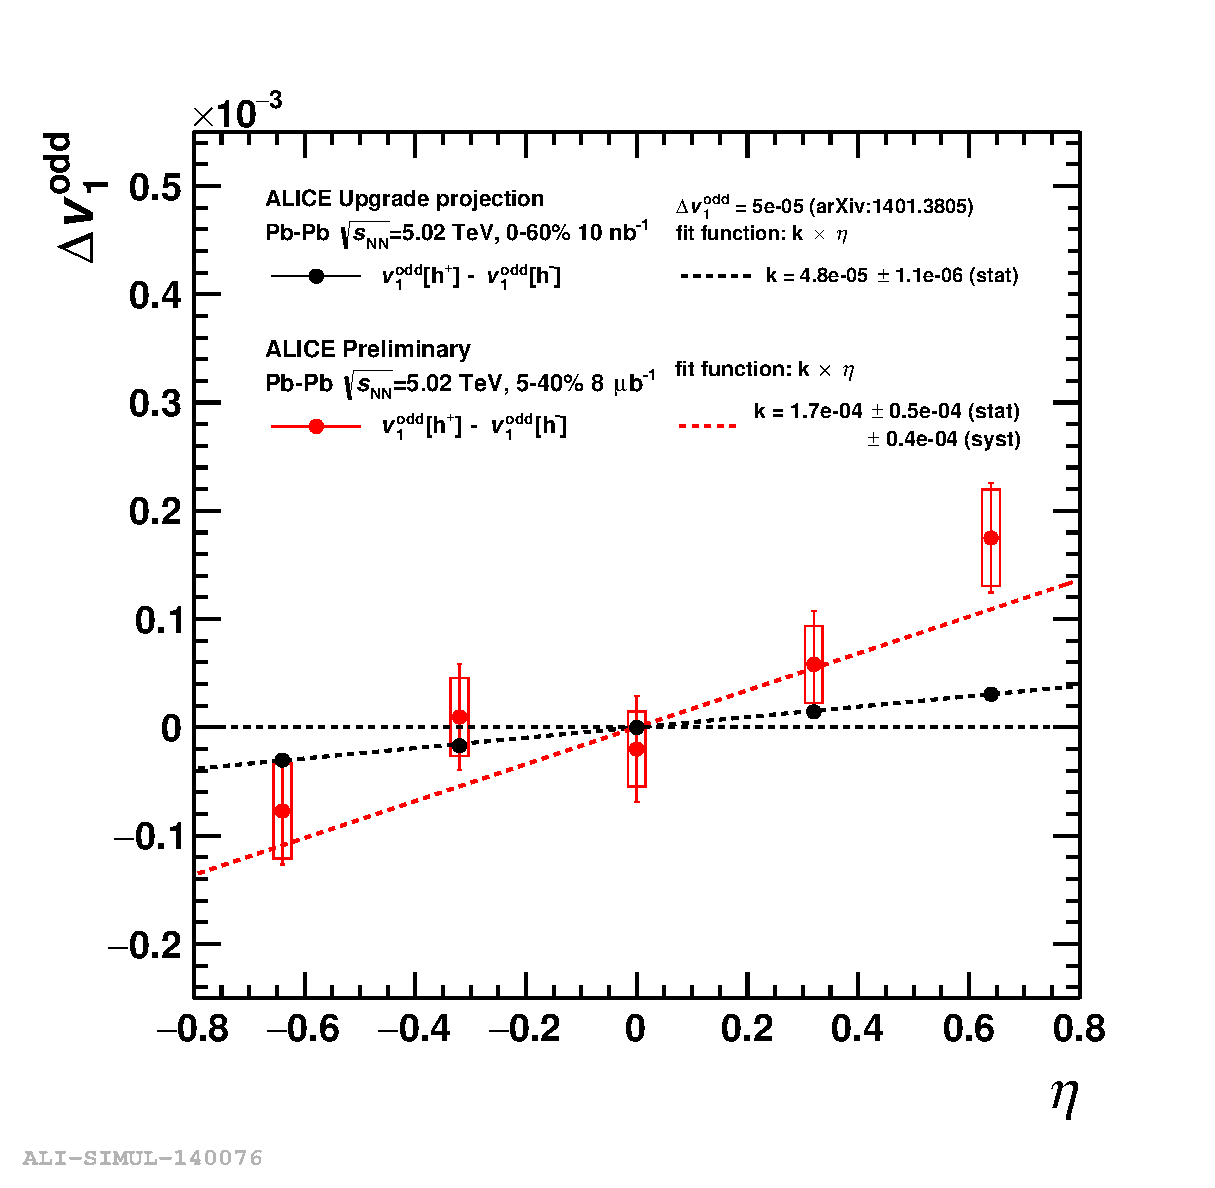
\includegraphics[width=0.8\textwidth]{figs/alice_projection_deltav1ch_stat8}
\caption{
}
\label{fig:alice_delta_v1}
\end{center}
\end{figure}


\begin{figure*}[!htb]
\begin{center}
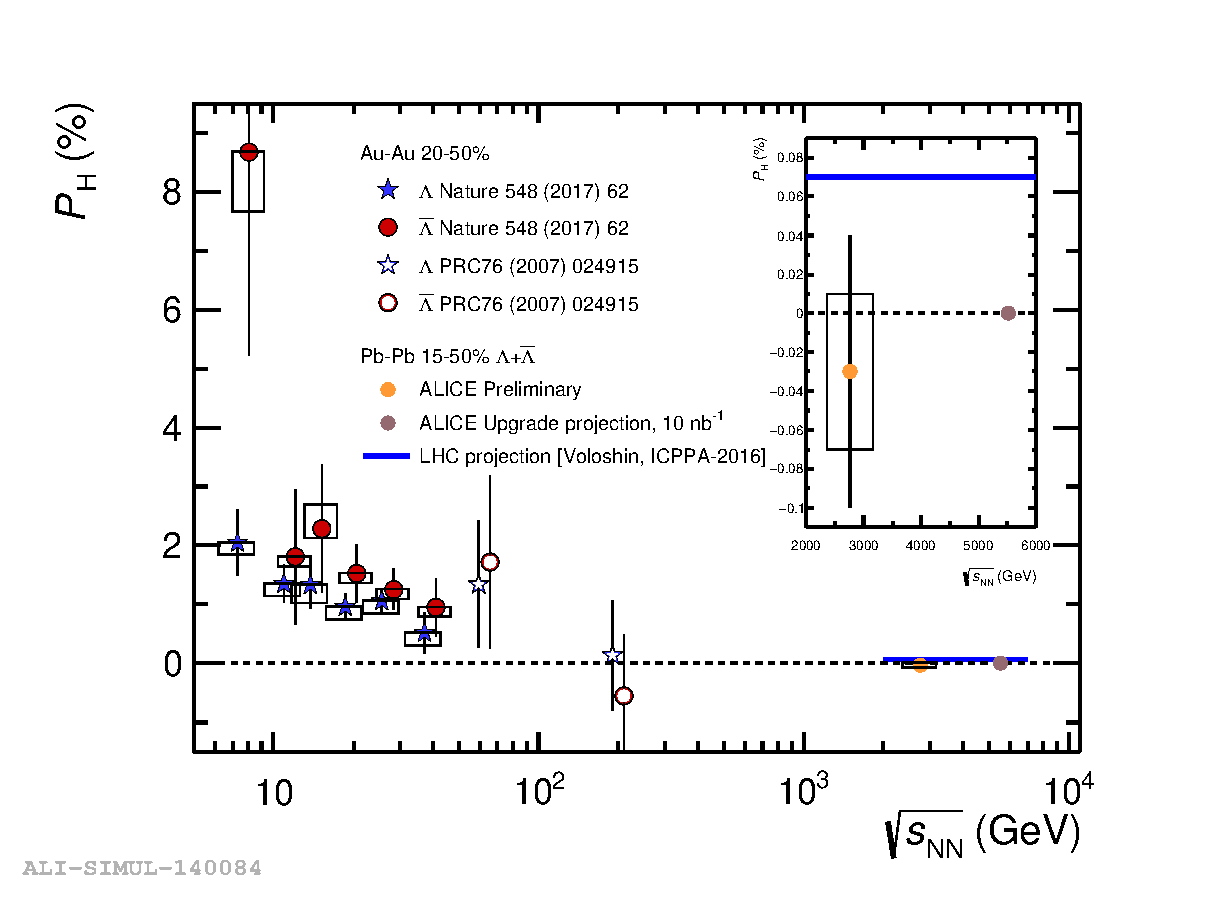
\includegraphics[width=0.8\textwidth]{figs/alice_projection_lambda}
\caption{Global polarization of $\Lambda$ and $\bar{\Lambda}$ as a function of the collision energy $\sqrt{s_{NN}}$ for semi-central heavy ion collisions. Open boxes
and vertical lines show systematic and statistical uncertainties,
respectively. Main panel: the data points for $\bar{\Lambda}$ are slightly horizontally shifted for visibility. Inner panel: the LHC energy domain is shown more detailed.
}
\label{fig:alice_lambda}
\end{center}
\end{figure*}

Fig. \ref{fig:alice_lambda} presents the energy dependence of the global polarization of $\Lambda$ and $\bar{\Lambda}$ for the semi-central heavy ion collisions. The RHIC results show the decrease of polarization at higher $\sqrt{s_{NN}}$. But $\Lambda$ and $\bar{\Lambda}$ demonstrate the finite global polarizations even at highest RHIC energy $\sqrt{s_{NN}}=200$ GeV \cite{PRC-98-014910-2018}. The preliminary ALICE data point at $\sqrt{s_{NN}}=2.76$ TeV is close in magnitude with results at $\sqrt{s_{NN}}=200$ GeV. But the ALICE upgrade projection at twice large collision energy corresponds to the zero polarization with very high precision. Therefore the study of global polarization of $\Lambda$ and $\bar{\Lambda}$ within HL--LHC project allows the unambiguous conclusion with regard of the values of this physics quantity in TeV-energy domain.    %Stefan,Alex
\FloatBarrier
\subsection{Chiral effects}

\begin{itemize}
	\item
The vacuum of quantum chromodynamics (QCD) is characterized by rich geometry structure which may corresponds to the fractal-like geometry \cite{IJMPE-22-1350041-2013}.There is a fundamental interrelation between geometry and essential properties of QCD Lagrangian.
Structures with non-trivial topology in QCD vacuum are believed to determine the behavior of the $\mathcal{P / CP}$ fundamental symmetries in the hot quark-gluon matter. Due to higher luminosity at the HL--LHC and / or high multiplicity per event at HE--LHC energy the multiparticle azimuthal correlations can be used for investigations of wide set of chiral effects in strong interaction \cite{PAN-80-1133-2017}, for instance, chiral magnetic effect -- CME, chiral magnetic waves -- CMW etc. This approach  allows the significant suppression of the backgrounds and improvement of reliability of physical conclusions. The study of charge-dependent azimuthal correlations for various types of light flavor particles can be possible with unprecedented precision due to high luminosity of the HL--LHC project. Consequently the quantitative comparison will be allowed for strengths of correlations in meson, baryon--meson and baryon systems. Such measurements will be essential in particular for search for chiral vortical effect -- CVE and its study with high precision. Furthermore the higher energies of the HE--LHC project can provide the opportunity for study of flavor dependence of the $\mathcal{P / CP}$ violation with help the azimuthal correlations for wider set of types of secondary particles including for heavy flavor ones. Thus experimental study of topology of QCD vacuum can be one of the focuses for studies of bulk properties within the HL--LHC, HE--LHC projects.
\end{itemize}



\begin{figure}[!htb]
\begin{center}
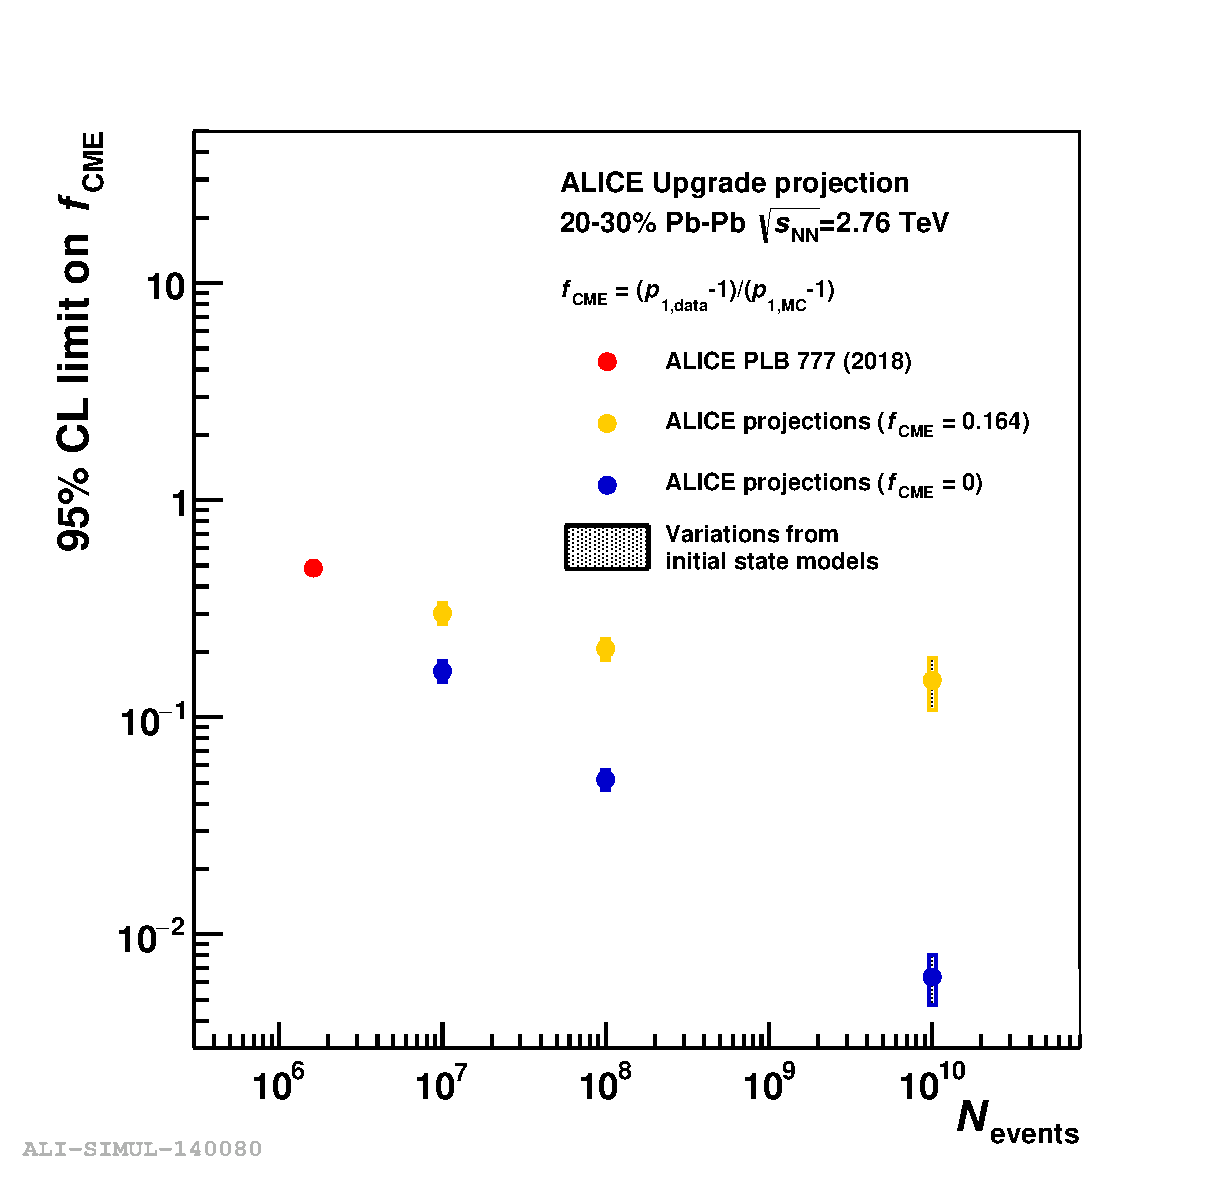
\includegraphics[width=0.8\textwidth]{\main/flow/figs/alice_projection_fcme}
\caption{
}
\label{fig:alice_fcme}
\end{center}
\end{figure}

 %Wei, Vitaly
\FloatBarrier
\subsection{Summary}
The measurements of inclusive hadron \vn\ by traditional methods such as 
  two-particle correlations, event-plane/scalar-product methods, 
  multi-particle cumulants etc. have been performed with high precision 
  by the ALICE, ATLAS and CMS experiments at the LHC.
These inclusive hadron \vn\ measurements are not statistically limited 
  across most of the centrality-\pt\ phase space and further improvement 
  in the measurements is not a high priority for Run~3 and 4.
However, in the case of identified hadrons the increased statistics 
  will lead to further improvement in the \vn\ measurements.
This is true for both light hadrons such as pions, protons, $\phi$-mesons 
  as shown in Figure~\ref{fig:alice_vn}, as well as for heavy-flavor 
  particles such as $D^0$, $D^{\pm}$, J/$\psi$, $\Upsilon$ which are 
  discussed in Chapters~\ref{sec:HI_HF} and \ref{sec:quarkonia}, respectively.
Significant improvements are expected in measurements of 
  longitudinal flow fluctuations, which have only been briefly investigated
  in Run~1 and 2.
These are largely driven by the increases $\eta$ acceptance of the
  ATLAS and CMS tracking detectors in Run~4, the acceptance is planned 
  to reach $\pm$5 units.
Other observables related to collective phenomena where current 
  measurements are statistics limited and are expected to improve 
  considerably are related to effects of vorticity and magnetic fields.

 %Soumya, Wei

\end{document}

